\subsection{Contrôle MIDI de LiveScaler}
Pour piloter LiveScaler, j'utilise un contrôleur MIDI composé d'une grille de $4\times 4$ touches. La figure \ref{fig:mapping-ATOM} montre la manière (le plus souvent appelée \emph{mapping}) dont les touches sont associées à des transformations de LiveScaler. 

\begin{figure}[htbp]
  \centering
  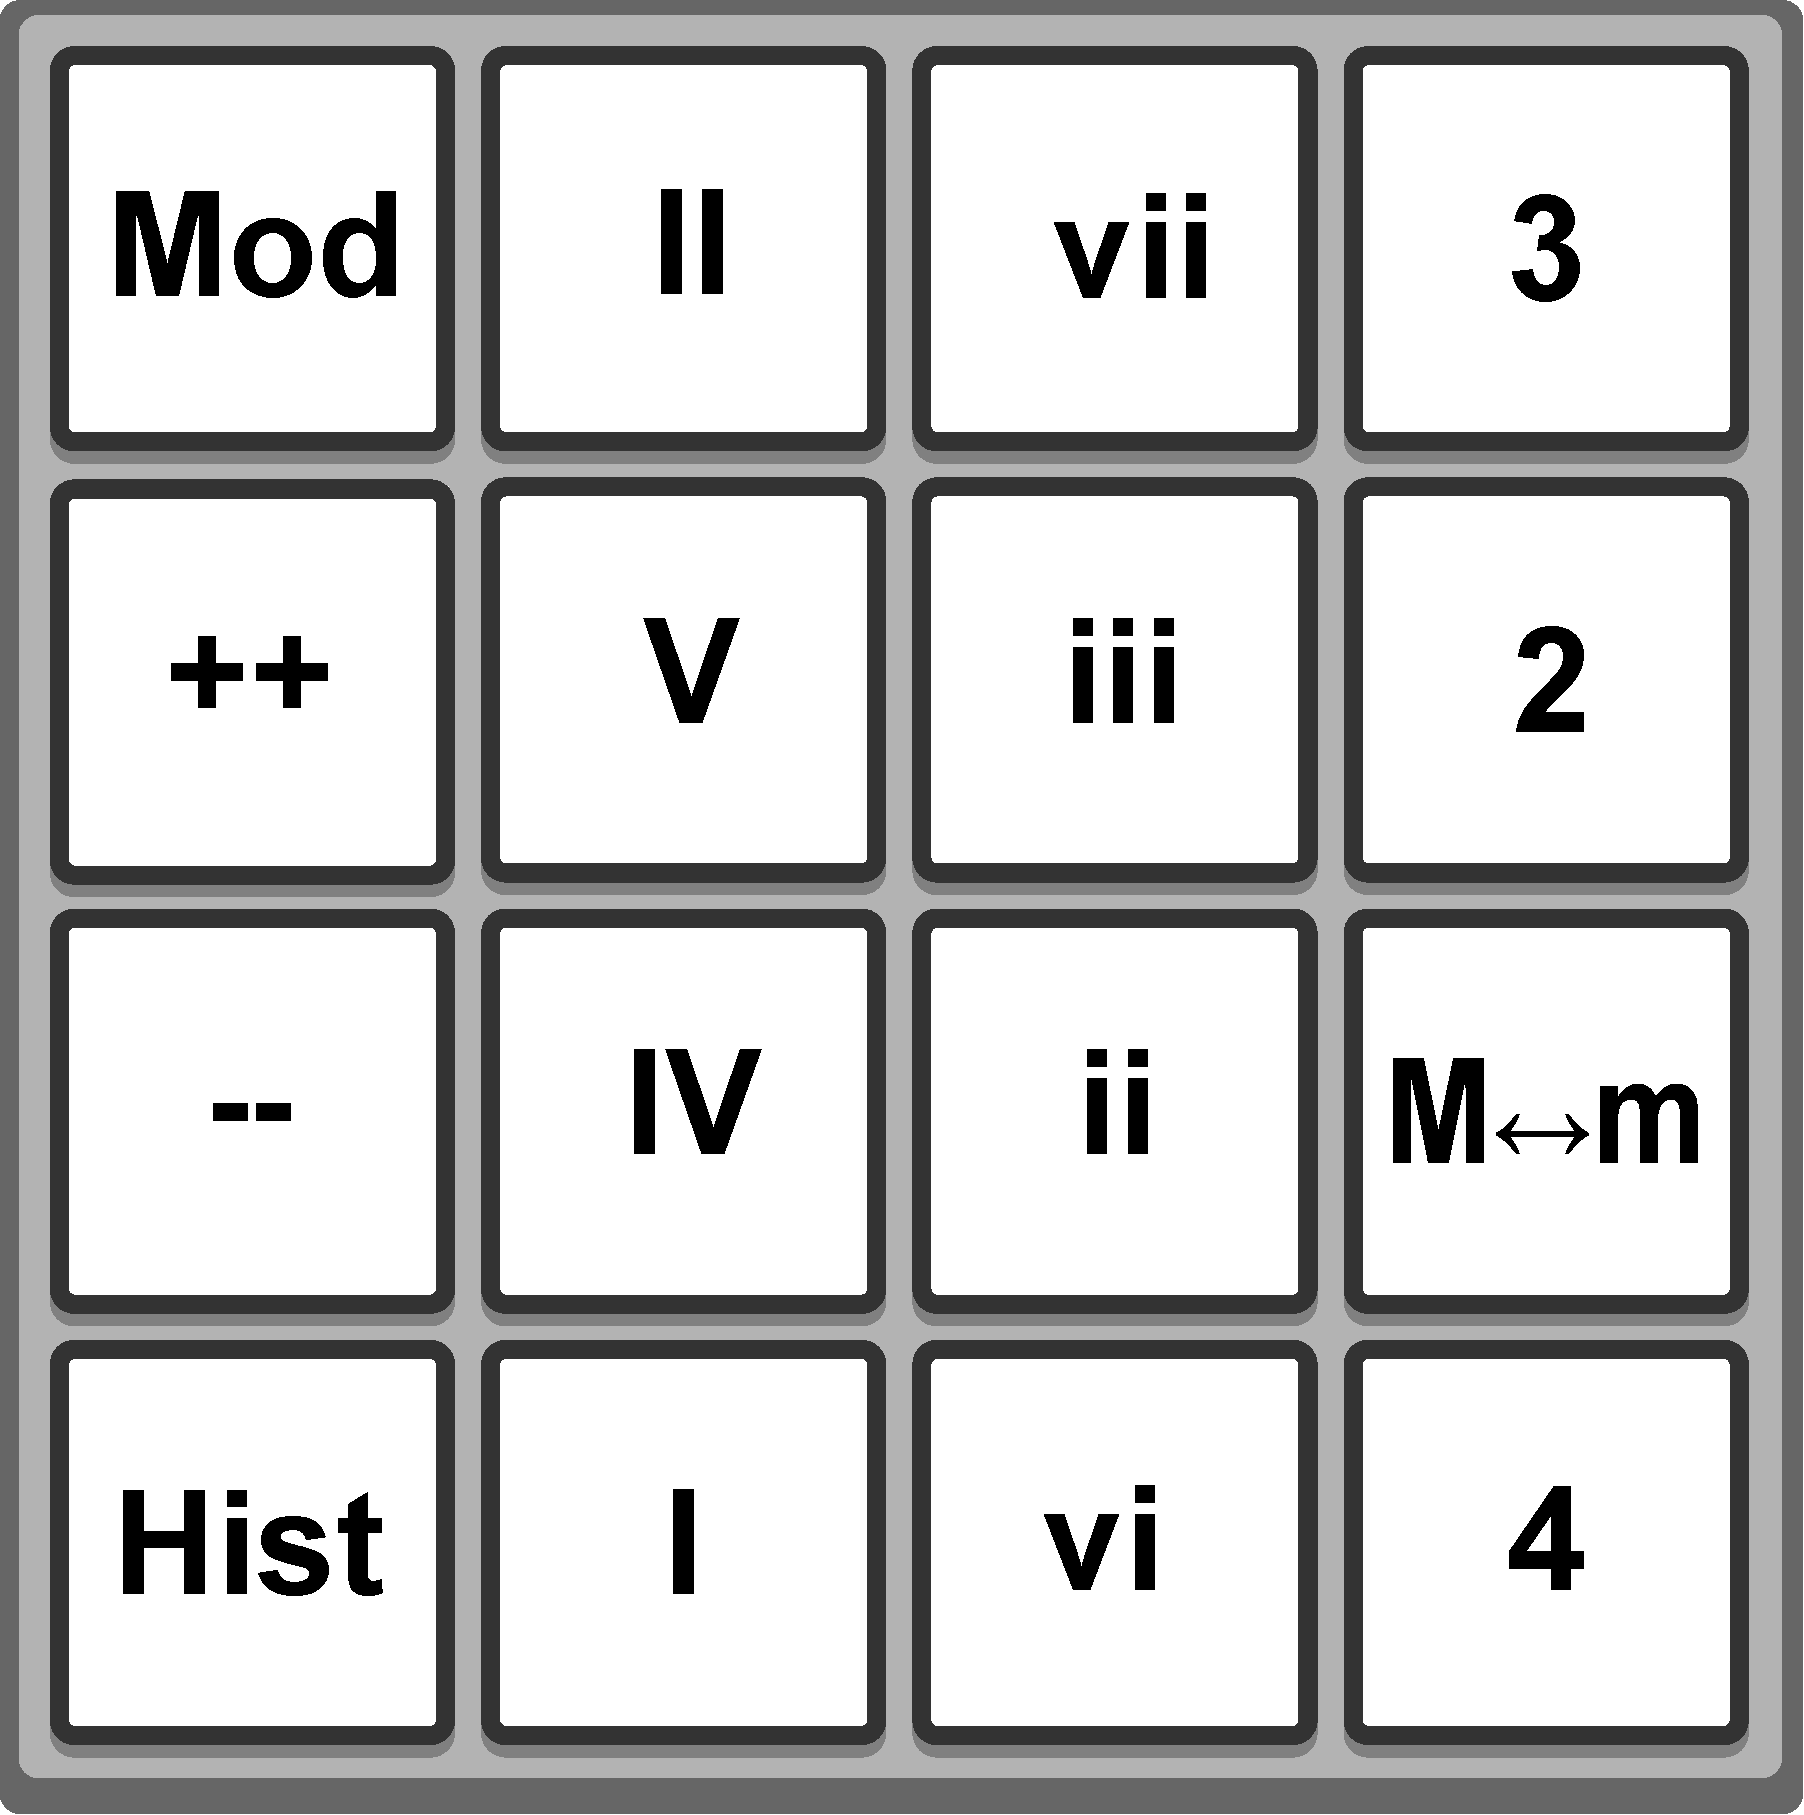
\includegraphics[width=0.55\textwidth]{Figures/Pads-config.pdf}
  \caption{Mapping de \emph{LiveScaler} sur un contrôleur MIDI à $4\times 4$ touches\label{fig:mapping-ATOM}}
\end{figure}

Voici le détail de l'action des différentes touches : 
\begin{itemize}
  \item \LSI,\LSvi,\LSIV,\LSII,\LSV,\LSiii,\LSII,\LSvii :  Les deux colones centrales déclenchent instantanément les transformations décrites précédemment. Elles sont organisées par relatives mineures/majeures.
  \item \texttt{Hist} : \emph{LiveScaler} garde en mémoire un court historique des transformation précédemment appliquées. Appuyer sur \texttt{Hist} permet de déclencher une des transformations de cet historique. Des combinaisons de la touche \texttt{Hist} et des touches \texttt{Hist}, \LSMm, $2$,$3$ et $4$ permettent de naviguer dans cet historique \footnote{Pour plus de détail, se référer au manuel de \emph{LiveScaler}}. 
  \item \LSpp, \LSmm : En combinant la touche $++$ (resp. $--$) avec une des transformations des colonnes centrales, on transpose cette transformation d'un demi-ton vers le haut (resp. vers le bas). 
  \item  \LSMm : permet de passer d'une transposition à une inversion et réciproquement. En pratique, combiner \LSMm avec \LSI (resp. \LSvi,\LSIV,\LSII,\LSV,\LSiii,\LSII,\LSvii) donnera la transformation \LSI (resp. \LSvi,\LSIV,\LSII,\LSV,\LSiii,\LSII,\LSvii).
  \item \LStwo,\LSthree,\LSfour : une combinaison de ces touches avec une des transformations des colonnes centrales permettent de modifier le coefficient modal de cette transformation.
  \item \LSMod : En combinant \LSMod avec une des transformations, on indique à \emph{LiveScaler} qu'on souhaite moduler l'harmonie de notre morceau vers cette nouvelle gamme. 
\end{itemize}

Ainsi, à partir d'une instrumentation jouant de manière répétée sur un accord de \writechord{C} majeur, on pourrait imaginer d'harmoniser en live cette instrumentation. Par exemple, si on veut reproduire la suite d'accord de la chanson Summer Nights de la comédie musicale Grease \footnote{Si, comme pour moi, cette chanson à tendance à rester dans votre tête, je suis (presque) désolée} en commençant par indiquer à \emph{LiveScaler} qu'on est dans une tonalité de Ré majeur (\LSMod + \LSII). Puis, une fois l'instrumentation lancée, on apuiera tous les deux temps sur, successivement $I ; IV ; V ; IV$.

Puis, arrivés au moment tant attendu de la modulation d'un demi-ton vers le haut,

\begin{tabular}{ccccc}
\LSI; & \LSIV; & \LSV; & \LSpp + \LSMm +  \LSvi; & \LSMod + \LSpp + \LSI
\end{tabular}
%$$I ; IV; V; \LSpp + (M\leftrightarrow m) vi; Mod + \LSpp + I$$

pour repartir joyeusement sur $I;IV;V;IV$, mais cette fois dans une tonalité de Mi bémol majeur. On aura ainsi obtenu la progression harmonique suivante : $$\dots - D - G - A - G - D - G - A - B\flat - E\flat -A\flat - B\flat - A\flat - \dots$$

\begin{comment}

L'objectif est de pouvoir communiquer une transformation affine via un contrôleur MIDI en un seul geste musical.


\begin{enumerate}
  \item Les distances sur le tonnetz sont similaires aux distances entre les pads
  \item Possibilité d'utilisation mélodique (on peut aisément jouer une gamme)
  \item Ancre : transposition et modulations (ajouter au cadre théorique ?)
  \item Historique : revenir aisément en arrière
\end{enumerate}
\end{comment}

